\begin{figure}
\centering
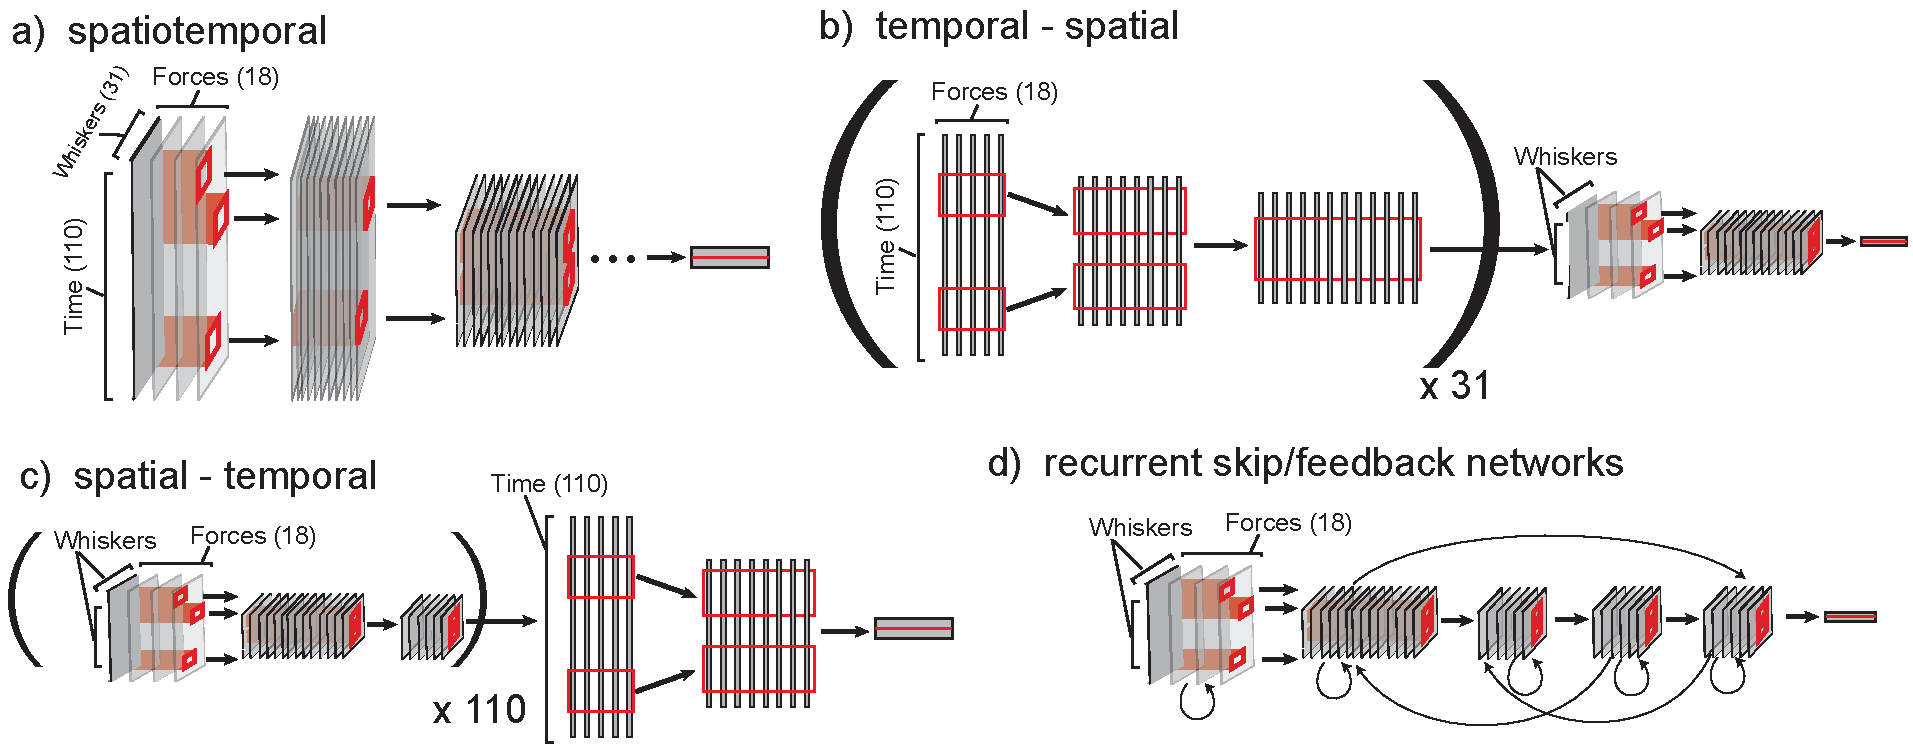
\includegraphics [width=1\linewidth]{figures/architectures.pdf}
\vspace{-2mm}
\caption{\textbf{Families of DNN Architectures tested:} \textbf{a.} Models with spatiotemporal integration at all stages. Convolution is performed on both spatial and temporal data dimensions, followed by one or several fully connected layers. \textbf{b.} Temporal-Spatial networks in which temporal integration is performed separately before spatial integration.  Temporal integration consists of one-dimensional convolution over the temporal dimension, separately for each whisker. the In spatial integration stages, outputs from each whisker are registered to their natural 2D spatial grid and spatial convolution performed.  \textbf{c.} In Spatial-Temporal networks, spatial convolution is performed first, replicated with shared weights across time points; this is then followed by temporal convolution. \textbf{d.} Recurrent networks with no explicitly separate units for handling for distinct timepoints, relying instead on state to build up memory traces.  These networks can have local recurrence (e.g. simple addition or more complicated motifs like LSTMs or GRUs), as well as long-range skip and feedback connections.~\label{fig_archi}}
\end{figure}

We trained deep neural networks of a variety of different architectural types on the shape-recognition task (Fig. \ref{fig_archi}).  
These architectures represent differing hypotheses about the computations performed by neurons in 
the subcortical and cortical areas downstream of the whisker follicles. 
The fundamental questions explored by these hypotheses are how and where temporal and spatial information are integrated.   


\subsection{Spatiotemporal integration}

In this family of networks, we use CNNs where convolution is done simultaneously on temporal dimension and spatial dimension, which means that responses from different whiskers across a specific window of time will be combined together in neurons of every layer, while neurons at higher layer will have larger receptive field at both dimensions.
We began with 2D-convolution on temporal and spatial dimension, where the spatial dimension is the indexing of the whiskers through going across the columns and then the rows on the $5\times7$ grid.
We also tried expanding the spatial dimension into two dimensions of $5\times7$ and then doing a 3D-convolution instead, the results will be shown later in this section.

The general structure of the networks includes several convolution layers followed by several fully connected layers. Each categorization is done towards a combination of top, middle, and bottom swipe of the same object under fixed setting.
The same network will be applied to three swipes after which the outputs will be concatenated to give the final categorization label.
For example, one structure in this family consists of 5 convolutional layers and 2 fully connected layers for each swipe with one additional fully connected layer for combining three swipes.
We will call this network as base network, whose structure will be described in detail below.
The convolutional layers of this network are named from \textit{conv1} to \textit{conv5}.
And the filter size of \textit{conv1} is $9\times3$ and that of other convolutional layers is $3\times3$, where the first number is for temporal dimension and the second number is for spatial dimension.
The strides of all convolutional layers for both dimensions are 1. The number of filters are 96, 256, 384, 384, and 256 respectively.
There are max-pooling layers after \textit{conv1}, \textit{conv2}, and \textit{conv5}, called \textit{pool1}, \textit{pool2}, and \textit{pool5}. The filter size of \textit{pool1} is $3\times1$ and the stride of \textit{pool1} is the same.
For \textit{pool2} and \textit{pool5}, the filter size is $3\times3$ while the stride is $2\times2$.
After \textit{pool5}, the output is transformed by two fully connected layers \textit{fc6} and \textit{fc7}. Layer \textit{fc6} has an output shape of 4096 and layer \textit{fc7} has an output shape of 1024.
Finally the three swipes are concatenated together and an additional fully connected layer \textit{fc\_add} is used to predict the category by giving an output with shape of 117.
The network is trained using cross-entropy loss function with Adagrad algorithm~\cite{duchi2011adaptive}.
And the learning rate remains at 0.01 for 15 epoches and then is adjusted to 0.005 for 10 extra epoches.

Several modifications are made to the base network for further explorations. First, two smaller networks with less parameters or even less layers are trained to check whether depth and parameters are necessary.
And as mentioned above, the base network with 3D-convolution rather than 2D-convolution is also trained.
Besides, there is only one additional layer combining the information from three swipes in the base network while the combined information could benefit from more layers of processing, so we also tried another network with more fully connected layers upon combined information.
Furthermore, the base network is only using top, middle, and bottom swipes of a fixed setting for categorization, while in the dataset, there are also three other groups of swipes towards the setting availabel, which means that the categorization could be done to 12 swipes. 
We tried one simple way to use this extra information. It is similar to that of combining information of three swipes. Specifically, we applied the same network to each swipe, concatenated all 12 swipes, and then used one additional layer to get the final label.


\subsection{Temporal integration first}

Instead of integrating spatial and temporal information at the begining, we could let the networks concentrate on processing temporal information for each individual whisker first and then combine the information from different whiskers in higher layers.
For each swipe, the networks in this family apply the same temporal convolutional network to the temporal signals of each whisker first. 
The outputs of each whisker are then reshaped into one dimension vectors individually and then reorganized in the grid of $5\times7$ according to the actual positions of each whisker with vacancies in the grid filled by zero vectors. 
Another spatial convolution network is applied after that to get a representation including both temporal and spatial information.
Finally, similar to the base network, we concatnate the information from three swipes and use an additional one-layer network to give the final label.

\subsection{Spatial integration first}

Similar to the previous section, while this time the inputs the spatial convolution is applied to 


\subsection{Fully recurrent networks}
